\documentclass[a4paper]{article}
\usepackage[utf8]{inputenc}
\usepackage[russian]{babel}
\usepackage[warn]{mathtext}

\usepackage{graphicx}
\usepackage{wrapfig}
\usepackage{amsmath}
\usepackage{floatflt}
\usepackage{float}
\usepackage{amssymb}
\usepackage{mathrsfs}

\usepackage{longtable}
\usepackage{multicol}
\usepackage{multirow}

\usepackage{lscape}
\usepackage{hvfloat}

\usepackage{indentfirst}

\usepackage[left=15mm, top=20mm, right=15mm, bottom=20mm, footskip=10mm]{geometry}
\linespread{1.3}
\usepackage{multicol}

\graphicspath{ {pic/} }

\begin{document}
\begin{titlepage}
\noindent

	\centering
	\vspace{2cm}
	{\scshape\LARGE Московский физико-технический институт (НИУ)\par}
	\vspace{1cm}
	{\scshape\Large Лабораторная работа\par}
	\vspace{1cm}
	{\huge\bfseries Волконный лазер\par}
	\vspace{1cm}
	
	\begin{figure}[H]
	\centering
	
\includegraphics[width=0.4\linewidth]{dpqe.jpg}
   	\label{fig:0}
	\end{figure}
	%\vspace{0.5cm}
	\vfill
	
\begin{flushright}
	{\large выполнили студенты III-ого курса ФФКЭ, группа 852}\par
	\vspace{0.3cm}
	{\LARGE Андреев Георгий} \par
	{\LARGE Анисимов Михаил} \par
	{\LARGE Бурков Александр} \par
	{\LARGE Водзяновский Яромир} \par
	\vspace{0.3cm}
	{\large преподаватель}\par
	\vspace{0.3cm}
	{\LARGE Юрий Юрьевич Брославец} \par
\end{flushright}

\vfill

% Bottom of the page
	Долгопрудный, 2020 г.
\end{titlepage}
\newpage
\tableofcontents
\newpage
\section{Цель работы}
\begin{itemize}
	\item рассмотреть теоретические вопросы, связанные с работой волоконных лазеров, а именно: процесс генерации в волоконном лазере, методы создания ин-версной заселенности, формирование модовой структуры лазерного излучения, фи-зические основы появления релаксационных колебаний;
	\item Экспериментально получить энергетические параметры выходного излу-чения, определить влияние параметров генерации на частоту и затухание релакса-ционных колебаний.
\end{itemize}

\section{Решение задач}
\begin{enumerate}
\item \textbf{Рассчитать частоту релаксационных колебаний для волоконного лазера, используемого в работе}.
Частота $\omega$ релаксационных колебаний лазера находится по формуле: 
\begin{displaymath}
\omega = \sqrt{\frac{x-1}{\tau_0 \tau}},
\end{displaymath}
где $x$ - превышение скорости накачки над пороговой, $\tau$ - время жизни рабочего уровня, $\tau_0$ - время жизни фотонов:
\begin{displaymath}
x = \frac{W_p}{W_{cp}} \hspace{2cm} \tau_0 = - \frac{2L}{c \cdot \ln(1-T)} = \frac{L'}{c\gamma},
\end{displaymath}
где $W_p$ - скорость накачки, $W_{cp}$ - критическая скорость накачки, $L$
 - длина резонатора, $c$ - скорость света, $T$ - коэффициент пропускания выходного зеркала, $L'$ - оптическая длина резонатора, $\gamma$ - потери в резонаторе за проход в одном направлении.
 
Данные: $x = 1,5; \tau = 1400 \mu sec; \tau_0 = 278 sec; $

Ответ: $\omega \approx 3,58 \cdot 10^4 \frac{rad}{sec}$
 
 
 \item \textbf{Определить время затухания фотонов в резонаторе волоконного лазера}
 
 Формула: $\tau_0 = \frac{L'}{c\gamma}$
 
 Данные: $L' = 10 metres, \gamma = 0,12;$
 
 Ответ: $\tau_0 \approx 278 ns$
 
 \item \textbf{Определить температуру, при которой работа иттербиевого лазера будет происходить по трехуровневой схеме, если штарковское расщепление уровней рабочего перехода $\approx 500 cm^{-1}$}
 
 В научной литературе энергию измеряют в обратных сантиметрах, которые характеризуют энергию электромагнитных квантов с соответствующей длиной волны. 
 
 Формула: $E = \frac{hc}{\lambda}, E \approx kT$. Следовательно, $T \approx \frac{hc}{k\lambda}$

 Ответ: $T \approx 720 K$.
 
 \item \textbf{Назовите условие генерации в любом лазере}
 Генерация в лазере возможна только при условии преобладания накачки энергии над ее потерями.
 
 \item \textbf{Возможна ли инверсная заселенность в двухуровневой системе?}
 Нет, невозможна. Если записать для двухуровневой системы скоростные уравнения и решить ее, то в результате получим $N < 0$ - плотность инверсной заселенности меньше нуля, что соответствует обычному, неинверсному состоянию активной среды.
 
 \item \textbf{Приведите сравнительную характеристику волоконных и твердотельных лазеров}
 
 
 \begin{table}[h]
	\begin{tabular}{|c|l|l|l|}
	\hline
	Хар-ка / лазер                    & \multicolumn{2}{l|}{Волоконный лазер}                                                                                                                                                                           & Твердотельный лазер                                                                                                                                                                   \\ \hline
	Активная среда                    & \multicolumn{2}{l|}{\begin{tabular}[c]{@{}l@{}}Сверхчистый плавленый кварц \\(основной материал оптоволокна), \\легированный ионами  редкоземельных\\ металлов-лантаноидов (\\ $Nd^{3+}, Yb^{3+}$)\end{tabular}} & \begin{tabular}[c]{@{}l@{}}Диэлектрический кристалл (н-р, \\ $Y_3Al_50_12$), стекло. \\ Центры – примесные ионы переходных \\ металлов (н-р $Cr^{3+}, Nd^{3+}, Er^{3+}$)\end{tabular} \\ \hline
	Система накачки                   & \multicolumn{2}{l|}{Широкополосные светодиоды, лазерные диоды}                                                                                                                                                  & Оптическая, лазерные диоды                                                                                                                                                            \\ \hline
	Резонатор                         & \multicolumn{2}{l|}{\begin{tabular}[c]{@{}l@{}}Р-р типа Фабри–Перо (на основе \\ диэлектрических зеркал, брэгговских\\  решеток), кольцевые р-ры\end{tabular}}                                                  & \begin{tabular}[c]{@{}l@{}}Растворы на основе диэлектрических \\ зеркал (разные типы)\end{tabular}                                                                                    \\ \hline
	\multirow{3}{*}{Спектр излучения} & $Nd^{3+}$: 0,92-0,94; 1,05-1,1; 1,34 $\mu m$                                                                    & $Ho^{3+}$: 1.9-2.1 $\mu m$                                                                    & \multirow{3}{*}{\begin{tabular}[c]{@{}l@{}}$CaF_2–Sm^{2+}$: 2.36 мкм(в общем, \\ частота меньше, чем у волоконных)\end{tabular}}                                                      \\ \cline{2-3}
									  & \textit{Er3+1.53-1.6 мкм}                                                                                       & \textit{Tm3+1.7-1.9 мкм}                                                                      &                                                                                                                                                                                       \\ \cline{2-3}
									  & \textit{Yb3+0.98-1.16 мкм}                                                                                      & \textit{-}                                                                                    &                                                                                                                                                                                       \\ \hline
	\end{tabular}
\end{table}
 
 
 
 
 
 
 
 
 
 
 
 
 
 
 
 
 
 
 
 
 
 
 
 
 
 
 \end{enumerate}

\section{Теоретические основы работы}
\subsection{Инверсия активной среды как необходимое условие генерации}

Излучение лазера рождается на переходах между определёнными энергетическими уровнями активных центров – рабочими уровня-ми. Отнесённые к единице объема активной среды заселённости рабочих уровней будем обозначать как n1 (нижний рабочий уро-вень) и n2 (верхний рабочий уровень). Разность

\begin{equation*}
N = n_2 - \frac{g_2}{g_1}n_1
\end{equation*}

Называют плотностью инверсной заселенности рабочих уровней. Где $g_1$ и $g_2$ - кратности вырождения соответсвующих уровней (будем полагать $g_1 = g_2$).
\par
Если выполняется $N>0$, имеет место инверсия активной среды. Понятие инверсии может относиться к определённым промежут-кам времени и областям активной среды. В термодинамически равновесной среде величина $N$ отрицательна. Обеспечение инвер-сии среды является необходимой предпосылкой для реализации режима генерации.

Коэффициент усиления активной среды описывается выражением:

\begin{equation*}
\chi_1 = \sigma N
\end{equation*}

где $\sigma$ - сечение вынужденных переходов между рабочими уровнями.

Активная среда так же харакетризуется линейным коэфицентом поглощения на неавктивных центрах и рассеяния $\chi_2$. Справедлив закон Бугера:

\begin{equation*}
dS_{\omega} = [\chi_1(z)-\chi_2(z)] S_{\omega}(z)dz
\end{equation*}

\subsection{Получение инверсной населенность с помощью когерентной оптической накачки}
Когерентная оптическая накачка предполагает возбуждение активных центров при поглощении активной средой излучения от специального источника.

Для ввода излучения накачки используется несколько методов:
\begin{enumerate}
\item Торцевой
\item Размещение V-бразных кановок по боковой поверхности светодиода
\item Два светодиода, размещенных в общей оболочке
\end{enumerate}

\subsection{Динамика генерации лазера}

Рассмотрим четерехуровневую схему генерации лазерного излучения, показанную на рис. \ref{fig:4_level}


\begin{figure}[H]
\centering
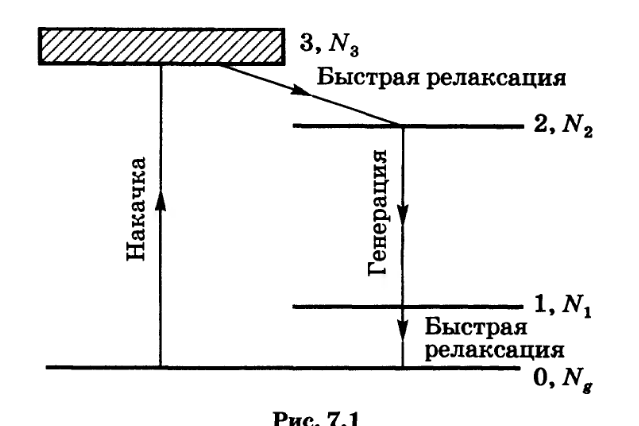
\includegraphics[width=0.5\linewidth]{4_level_scheme.png}
\caption{Четырехуровневая схема}
\label{fig:4_level}
\end{figure}

Считая, что переходы между 3 и 2, 1 и g являются быстрыми, положим $n_3 = n_1 \approx 0$. В этом случае скоростные уравнения можно записать следующим образом:
\begin{equation*}
\begin{cases}
\frac{dn_2}{dt} = W_p n_g - Bqn_2 - \frac{n_2}{\tau} \\
\frac{dq}{dt} = V_a B q n_2 - \frac{q}{\tau_c} \\
n_g + n_2 = N_t
\end{cases}
\end{equation*}

Где $q$ - полное число фотонов в резонаторе, $W_p$ - скорость накачки. $\tau = 1400$ мкс - время жизни рабочего уровня. $\tau_c = \frac{L'}{c \gamma}$ - время жизни фотонов в резонаторе; $\gamma$ - потери в резонаторе за переход в одном направлении; $V_a = \frac{\pi \omega_0^2 l}{4}$ - объём моды в активной среде; $L' = L + (n_0-1)l$. 

Вводя инвернсую заселенность уровней ($N = n_2 - n_g \approx n_2 $) представим систему в виде:

\begin{equation*}
\begin{cases}
\frac{dN}{dt} = W_p (n_2 - N) - BqN - \frac{N}{\tau} \\
\frac{dq}{dt} = V_a B q N - \frac{q}{\tau_c}
\end{cases}
\end{equation*}

Определим пороговое условие генерации. Пусть в момент времени $t = 0$ в резонаторе присутсвует некторое число фотонов $q$. Чтобы величина $\frac{dq}{dt}$ была положительной, должно выполняться $V_a BN - \frac{q}{\tau_c} > 0$. В этом случае генерация возникнет если $N$ достигает некоторого граничного значения, определяемого как:

\begin{equation*}
N_C = \frac{1}{V_a B \tau_c} = \frac{\gamma}{\sigma l'}
\end{equation*}

Критическая (пороговая) скорость накачки соответствует ситуации, когда полная скорость накачки уровней уравновешивает скорость спонтанных переходов с рабочего уровня.

\subsection{Релаксационные колебания}

Рассмотрим работу лазера при нестационарной накачке. Для данной временной зависимости скорости накачки $W_p(t)$ можно найти временную зависимость $q(t)$ и $N(t)$, если заданы начальные условия.

В случае, когда скорость накачки описывается ступенчатой функцией, будем считать, что скорость накачки имеет следующую временную зависимость: $W_p(t)$ = 0 при $t<0$ и $W_p(t) = W_p$ с независящей от времени величиной $W_p$ при $t>0$. При небольших колебаниях инверсии и количества фотонов около стационарных значений $N_0$ и $q_0$ можно записать:

\begin{displaymath}
\begin{cases}
N(t) = N_0 + \delta N \\
q(t) = q_0 + \delta q , 
\end{cases}
\end{displaymath}
где $\delta q << N_0$ и $\delta q << q_0$. Тогда можно получить систему:
\begin{displaymath}
\begin{cases}
\delta \dot{N} = - \delta N(W_p + \frac{1}{\tau}) - B(q_0 \delta N + N_0 \delta q) \\
\delta \dot{q} = B q_0 V_a \delta N
\end{cases}
\end{displaymath}

С учетом $B V_a N = \frac{1}{\tau_c}$, имеем уравнение колебаний:
\begin{equation*}
\delta\ddot{q} + [W_p + \frac{1}{\tau} + Bq_0]\delta\dot{q} + (B^2N_0q_0V_a)\delta q = 0
\end{equation*}
Решение имеет вид: $\delta q = \delta q_0 \exp(st)$
В этом случае получаем уравнение на параметр $s$:
\begin{equation*}
s^2 + (2/t_0)s + \omega^2 = 0
\end{equation*}
где $\omega^2 = B^2N_0q_0V_a$, $\frac{1}{t_0} = \frac{1}{2}(W_p +\frac{1}{\tau} + Bq_0 )$. Для случая $\frac{1}{t_0} << \omega$ получаем
\begin{equation*}
s = - \frac{1}{t_0}\pm i\omega'
\end{equation*}
\begin{equation*}
\omega'^2 = \omega^2 - \frac{1}{\tau_0}^2
\end{equation*}

В этом случае решение будет представлять собой затухающее гармоническое колебание 
\begin{equation*}
\delta q = C exp(-t/t_0)sin(w't + \phi),
\end{equation*}
где константы $C, \phi$ определяются начальными условиями. Для изменения инверсии в случае $1/t_0 << \omega'$ имеем:
\begin{equation*}
\delta N = \frac{\omega' C}{Bq_0V_a} exp(-t/t_0)sin(w't + \phi),
\end{equation*}
Выражения для $t_0$ и $\omega$ можно записать в более простом виде:
\begin{equation*}
t_0 = \frac{2\tau}{x}, \hspace{2cm} \omega = \sqrt{\frac{x-1}{\tau_c \tau}}, 
\end{equation*}
где $x = W_p / W_{cp}$ - превышение скорости накачки над пороговой. Таким образом, при ступенчатом включении накачки при генерации лазера происходят затухающие релаксационные колебания количества фотонов в резонаторе и, следовательно, выходной мощности с частотой $\omega'$.




\newpage

\section{Экспериментальная часть}
\subsection{Схема установки}
Схема установки представлена на рисунке \ref{fig:scheme}

\begin{figure}[H]
\centering
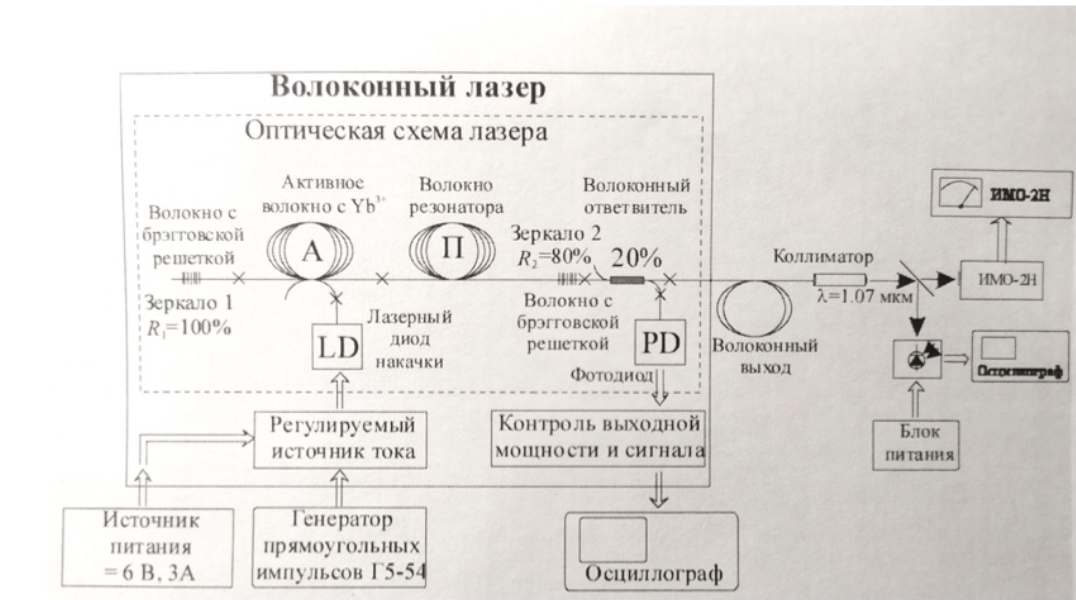
\includegraphics[width=0.8\linewidth]{scheme.png}
\caption{Блок-схема экспериментальной установки}
\label{fig:scheme}
\end{figure}

На схеме изображены:
\begin{itemize}
\item Волоконный лазер;
\item Источник питания;
\item Генератор Г5-54;
\item Измеритель энергии ИМО-2н;
\item Делительная пластинка;
\item Фотодетектор ФД-24К;
\item Осциллограф;
\item Источник питания фотодектора.
\end{itemize}

\subsection{Зависимость мощности излучения от мощности накачки}

С помощью заранее прокалиброванного калориметра, амперметра и вольтметра снимем график зависимости мощности излучения от мощности накакачки, представленный на рис. \ref{fig:P_vs_P}


\begin{figure}[H]
\centering
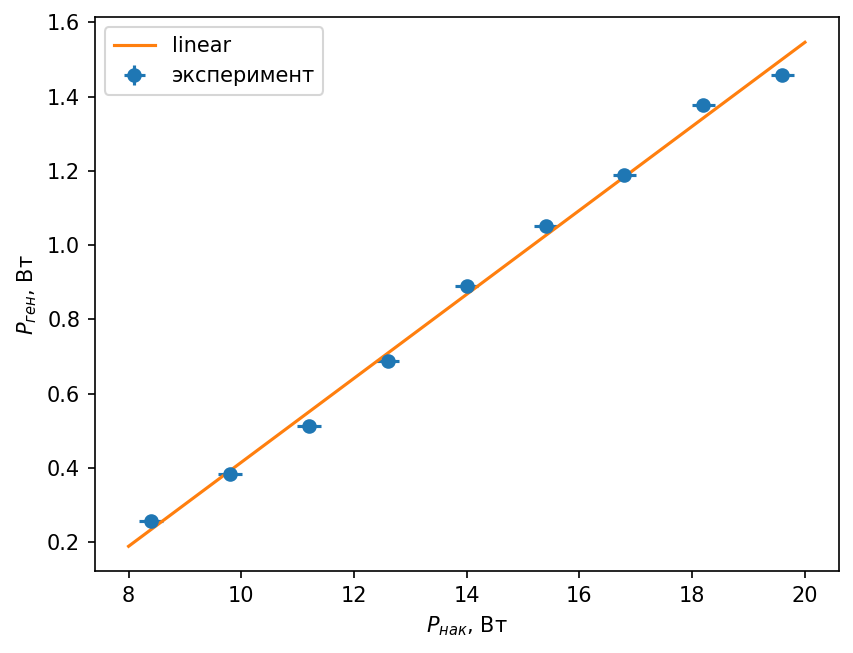
\includegraphics[width=0.5\linewidth]{P_vs_P.png}
\caption{график мощности излучения от мощности накачки}
\label{fig:P_vs_P}
\end{figure}

По графику получаем значение для кпд $\nu = 11.31 \pm 0.03 $ \% \par
И пороговую мощность: $P_{\text{порог}} = 6.33 \pm 0.01$ Вт

\subsection{Зависимость частоты релаксационных колебаний от превышения над порогом}

Используя цифровой осцилограф найдем период релаксационных колебаний и замеряем мощность накачки.

В данной эксперименте ожидаем зависимость:

\begin{equation}
\omega = \sqrt{\frac{x-1}{\tau_c \tau}}
\end{equation}

где $x = P/P_{\text{порог}}$

Построим график в единицах $(x-1)^{1/2}$, $f$ представленный на рис \ref{fig:x_vs_f}

\begin{figure}[H]
\centering
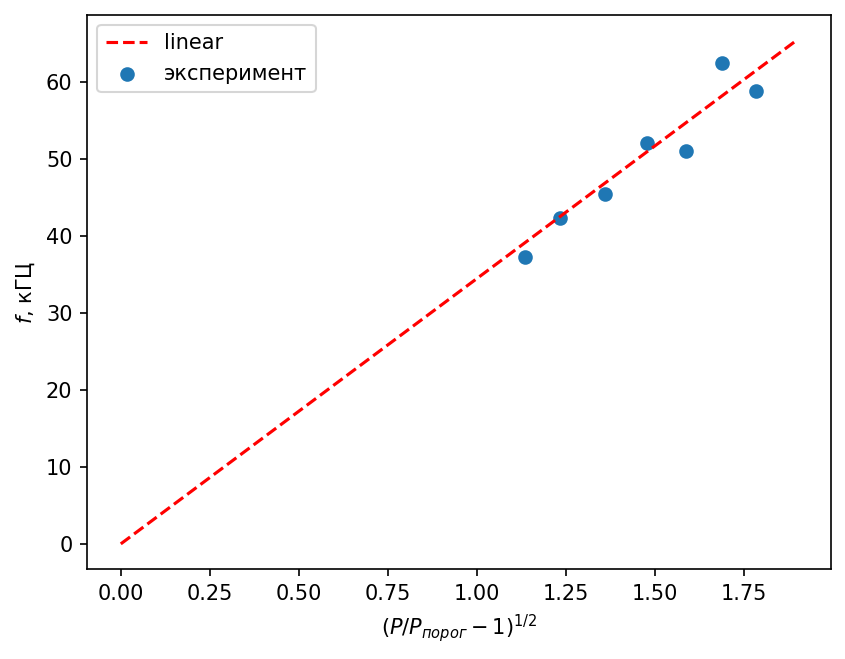
\includegraphics[width=0.5\linewidth]{x_vs_f.png}
\caption{график зависимости частоты релаксационных колебаний}
\label{fig:x_vs_f}
\end{figure}

Из коэффицента наклона, при $\tau_c = 27$ нс получаем: $\tau = 0.070 \pm 0.007$ мс.

Т.е. характерное время затухания релаксационных колебаний для известной мощности ступенчатой накачки определяется как $t_0 = 0.14/x$ мс
\newpage
\section{Выводы}
\begin{itemize}
\item Познакомились с основами теории волоконных лазеров: процессом генерации, методом создания инверсной заселенности и явлением релаксационных колебаний
\item  Измерили кпд и пороговую мощность волоконного лазера
\item Проверили зависимость частоты релаксационных колебаний от мощности накачки. Нашли коэфицент связывающий время затухание и превышение над порогом мощности.
\end{itemize}


\end{document}